\documentclass[answers, a4paper, 11pt]{exam}
\usepackage{amsmath}
\usepackage{amssymb}
\usepackage{amsthm}
\usepackage[italian]{babel}
\usepackage{ccicons}
\usepackage{hyperref}
\usepackage{cleveref}
\usepackage[utf8]{inputenc}
\usepackage[autostyle=false, style=english]{csquotes}
\usepackage[margin=2cm]{geometry}
\usepackage{graphicx}
\usepackage{mathrsfs}
\usepackage{multicol}
\usepackage{relsize}
\usepackage{parskip}
\pagestyle{plain}
\graphicspath{{./images/}}
\MakeOuterQuote{"}
\setlength{\columnseprule}{.4pt}
\renewcommand{\solutiontitle}{\noindent\textbf{R:}\enspace}
\def\dbar{{\mathchar'26\mkern-12mu d}}
\title{Fondamenti di Intelligenza Artificiale M}
\author{Kevin Michael Frick}
\begin{document}
\maketitle
\textbf{Titoli di testa}: Ringrazio di cuore Corinna, Davide e Antony per l’aiuto nella stesura di questo documento, nella preparazione di questo esame e per aver partecipato con me alla Tablut Challenge. Vi si vuole bene ragazz*.
\begin{questions}
\question Si dia la descrizione di ricerca iterative deepening, anche in pseudo-codice. Si discutano le sue
proprietà (in termini di completezza, ottimalità e complessità sia spaziale sia temporale).
	\begin{solution}
		Per evitare che la ricerca in profondità si perda in strade infinite è possibile limitarne la profondità, ovvero impostare un limite $l$ e smettere di esplorare una volta raggiunto un nodo con profondità $l$.
		La complessità temporale diventa allora $O(b^l)$ e quella spaziale $O(bl)$. 
		Se, però, il valore di $l$ è scelto male l'algoritmo non potrà raggiungere una soluzione. 
		Per questo motivo ci si serve della \emph{ricerca iterative deepening}, che consiste nel lanciare ripetutamente una ricerca in profondità con valori di $l$ che incrementano progressivamente finché non viene trovata una soluzone. 
		La complessità spaziale è $O(bd)$ in presenza di una soluzione o $O(bm)$ in uno spazio degli stati finito senza soluzione. 
		La ricerca iterative deepening è ottimale per problemi nei quali tutte le azioni hanno lo stesso costo ed è completa in tutti gli spazi degli stati finiti e aciclici, o nei quali il controllo dei cicli coinvolge l'intero cammino. 
		La complessità temporale è $O(b^d)$ in presenza di una soluzone e $O(b^m)$ in sua assenza. 
		Ogni iterazione genera un nuovo livello, ma a differenza della ricerca in ampiezza i livelli precedenti vengono ricalcolati, risparmiando memoria al costo di maggiore tempo. 
		La ricerca in ampiezza può sembrare molto dispendiosa perché gli stati vicini alla radice dell'albero di ricerca sono rigenerati più volte. 
		Tuttavia, in molti spazi degli stati la maggior parte dei nodi sono nei livelli più bassi, quindi questa rigenerazione non è molto rilevante. 
		La ricerca iterative deepening è da preferire quando lo spazio degli stati non sta nella memoria e la profondità della soluzione non è nota. 
	Lo pseudocodice per la ricerca iterative deepening è il seguente:
\begin{verbatim}
function iterative_deepening_search(problem) returns solution or failure
  for depth from 0 to inf do
    result <- depth_limited_search(problem, depth)
    if result != cutoff then return result

function depth_limited_search(problem, max_depth) returns node or failure or cutoff
  frontier <- new stack
  push(frontier, problem.initial_node)
  result <- failure
  while frontier is not empty do:
    node <- pop(frontier)
    if is_goal(problem, node) then return node
    if depth(node) > max_depth then result <- cutoff
    else if not is_cycle(node) do
      for each child in expand(problem, node) do
        push(frontier, child)
  return result
\end{verbatim}
	\end{solution}
\question Si discutano gli algoritmi di consistenza di una rete CSP e in particolare si descriva (in pseudocodice) l’algoritmo di arc-consistenza.
  \begin{solution}
    Un CSP è definito come un insieme di variabili $x_k$ e domini $D_k$ tali che $x_k \in D_k \forall k \in 1..n$ e di vincoli $c_k(x_{i1}, ..., x_{ij}) \subseteq D_{i1} \times ... \times D_{ij}$ su $j$. 
    I vincoli solitamente sono rappresentati in termini di relazioni. 
    Trovare una soluzione a un CSP prevede un assegnamento di tutte le $x_k$ che soddisfi tutti i vincoli $c_k$. 

    Gli algoritmi di consistenza rappresentano il probleam come un grafo di vincoli. 
    Gli archi possono essere orientati o meno a seconda del tipo di relazione: a relazioni non simmetriche corrispondono archi orientati, a relazioni simmetriche archi non orientati o doppiamente orientati. 
    I vincoli unari sono rappresentati da archi che iniziano e terminano sullo stesso nodo. 
    Gli algoritmi di consistenza riducono il problema eliminando dai domini delle variabili i valori che non possono comparire in una soluzione finale. 
  La node-consistency, o consistenza di grado 1, richiede che ogni valore $x_k \in D_k$ soddisfi i vincoli unari su $x_k$. 
    Per rendere consistente un nodo è necessario eliminare dal dominio di $x_k$ i valori che violano i vincoli. 
    Un grafo è consistente se lo sono tutti i suoi nodi. 
    L'arc-consistency, o consistenza di grado 2, si ottiene partendo da un grafo node-consistent. 
    Un arco $A(i, j)$ è consistente se per ogni valore $x \in D_i$ esiste almeno un $y \in D_j$ tale che il vincolo $c(i, j)$ tra $i$ e $j$ sia soddisfatto. 
    La rimozione di alcuni valori dal dominio di una variabile rende necessarie ulteriori verifiche che coinvolgono i vincoli contenenti la stessa variabile, quindi si rende necessario ripetere il procedimento di rimozione fino a che la rete non raggiunge uno stato di \emph{quiescenza}. 
    Il controllo della consistenza di un arco può essere applicato come passo di propagazione dopo ogni assegnamento. 
    In questo caso si parla di \emph{maintaining arc-consistency} (MAC). 
    L'algoritmo completo per il controllo di consistenza si chiama AC-3. 
    AC-3 si serve di uan coda di archi alla quale, ogni volta che il dominio di una variabile $x_i$ viene ridotto, vengono aggiunti gli archi $A(x_k, x_i)$ per ogni variabile $x_k$ collegata da un arco incidente su $x_i$. 
    Lo pseudocodice di AC-3 è il seguente: 
\begin{verbatim}
function ac3(csp) returns csp
  q <- new queue
  for each arc in csp do:
    push(q, arc)
  while q is not empty do:
    xi, xj <- pop(q)
    if remove_inconsistent_values(xi, xj) then:
      for each xk in expand(csp, xi) do:
        push(q, (xk, xi))
  return csp

function remove_inconsistent_value(xi, xj) returns boolean
  removed <- false
  for each x in domain(xi) do:
    if not exists y in doman(xj) s.t. (xi, xj) is satisfied then:
      delete(domain(xi), x)
      removed <- true
  return removed
\end{verbatim}
  \end{solution}

\question Si introduca il trattamento della negazione in Prolog. Si spieghi la differenza con la negazione
classica ed i problemi che può introdurre. Si mostri poi la sua realizzazione in Prolog.
\begin{solution}
  La negazione classica, che è anche quella utilizzata nelle basi di dati, è basata sulla CWA (Closed World Assumption) in cui se un atomo "ground" A non è conseguenza logica di un programma P, allora si può inferire $\sim A$.
  Tuttavia non esiste alcun algoritmo in grado di stabilire in un tempo finito se A non è conseguenza logica di P a causa dell'indecidibiltà (semi-decidibilità) della logica del primo ordine. Attraverso l'aggiunta di nuovi assiomi alla teoria, infatti, si può modificare l'insieme di teoremi che valeva precedentemente.
  È proprio per questo motivo che Prolog, così come ogni altro linguaggio logico, adotta una negazione per fallimento ("Negation as Failure" - NF). Essa si limita a derivare la negazione di atomi la cui derivazione termina con fallimento finito.
  In particolare, i sistemi Prolog si basano sulla cosiddetta risoluzione SLDNF: per dimostrare $\sim A$, dove A è un atomo, l'interprete del linguaggio cerca di costruire una dimostrazione per A.
  Se la dimostrazione ha successo, allora la dimostrazione di $\sim A$ fallisce. Se, invece, la dimostrazione per A fallisce finitamente si considera $\sim A$ dimostrato con successo.
  Il problema derivante da questa impostazione è una errata interpretazione dei quantificatori nel caso di letterali non "ground".
  Si consideri il seguente programma:
  \begin{verbatim}
    capitale(roma).
    capoluogo(bologna).
    citta(X) :- capitale(X).
    citta(X) :- capoluogo(X).
  \end{verbatim}
  E si consideri, a questo punto, il goal G:
  \begin{equation*}
    \exists X \sim capitale(X).
  \end{equation*}
  Esiste una entità che non è capitale, ovvero Bologna.
  Con la risoluzione SLDNF si cerca una dimostrazione per:
  \begin{equation*}
    F = \exists X capitale(X).
  \end{equation*}
  Dopo che si nega il risultato si ottiene:
  \begin{equation*}
    \sim F = \sim(\exists X capitale(X)).
  \end{equation*}
  Che corrisponde a:
  \begin{equation*}
    \sim F = \forall X (\sim capitale(X))
  \end{equation*}
  Quindi se esiste una X che è capitale, $\sim F$ fallisce, ma la query originaria era:
  \begin{equation*}
    F= \exists X \sim capitale(X).
  \end{equation*}
  Ovvero dimostrare che esiste X che non è capitale, che è una query ben diversa.
  Si rifletta, inoltre, sul fatto che Prolog adotta una regola di selezione dei letterali left-most (non safe). Questo può generare problemi perchè il significato logico di tali query è diverso da quello atteso.
  A tal proposito si consideri il seguente programma:
  \begin{verbatim}
    disoccupato(X) :- adulto(X), \+(occupato(X)).
    occupato(giovanni).
    adulto(mario).
  \end{verbatim}
  Si riportano due query e le relative risposte da parte del programma:
  \begin{verbatim}
    ?- \+(occupato(giovanni)).
    -> no
    ?- \+(occupato(mario)).
    -> yes
  \end{verbatim}
  Alla seguente query si ottiene la relativa risposta:
  \begin{verbatim}
    ?- disoccupato(X).
    -> yes X=mario
  \end{verbatim}
  A questo punto consideriamo lo stesso programma, ma con i due sottogoal nel corpo della clausola scambiati:
  \begin{verbatim}
    disoccupato(X) :- \+(occupato(X)), adulto(X).
    occupato(giovanni).
    adulto(mario).
  \end{verbatim}
  E la risposta alla query:
  \begin{verbatim}
    ?- disoccupato(X).
    -> no
  \end{verbatim}
  La risposta è no, perché scambiando i letterali, il letterale negativo viene selezionato quando è ground.
  Per questo è buona regola di programmazione verificare che i goal negativi siano sempre ground al momento della selezione.


  In Prolog è possibile aggiungere al database predicati negati mediante l'operatore \texttt{\textbackslash +}. 
  Ad esempio, per asserire che ``un adulto è disoccupato se non è occupato'' è possibile asserire 
  \begin{verbatim}
  disoccupato(X) :- adulto(X), \+occupato(X).
  adulto(giovanni).
  occupato(mario).
  \end{verbatim}
  A questo punto, la query otterrà il risultato atteso:
  \begin{verbatim}
?- disoccupato(giovanni).
true.

?- disoccupato(mario).
false.

  \end{verbatim}
  Una possibile implementazione della negazione in prolog è la seguente: \newline
  \begin{verbatim}
    not(A):- call(A), !, fail.
    not(A).
  \end{verbatim}
  Si noti l'utilizzo del metapredicato fail che forza il fallimento di una dimostrazione dell'interprete prolog.
    \end{solution}


\question Dare il significato di euristica ammissibile, e enunciare le proprietà che ne derivano per l’algoritmo
di ricerca A* che utilizzi una tale euristica.
	\begin{solution}
		Un'euristica $h(x)$ è ammissibile se, essendo $d(x)$ la vera distanza di un nodo $x$ dal nodo di arrivo e $V$ l'insieme dei nodi di un grafo, si ha $h(x) \leq d(x) \forall x \in V$, ovvero l'euristica è \emph{ottimistica}. 
		Se la ricerca A* utilizza un'euristica ammissibile allora è garantito che restituirà la soluzone ottimale. 
	\end{solution}
\question Si confrontino in maniera concisa le proprietà (complessità spaziale, temporale, ottimalità e completezza) delle strategie di ricerca non informate.
\begin{solution}
  Le strategie di  ricerca non informate sono la ricerca in profondità (DFS), la ricerca in ampiezza (BFS), la DFS a profondità limitata e la ricerca iterative deepening. 

  La BFS ha complessità temporale e spaziale $O(b^d)$ essendo $d$ la profondità e $b$ il fattore di ramificazione.
  La BFS è completa ma difficile da implementare efficientemente su architetture monoprocessore.
  La BFS, infine, trova il cammino a costo minimo solo se il costo di ogni nodo coincide con la profondità. 
  In caso contrario è necessario applicare la ricerca a costo uniforme, o algoritmo di Dijkstra, che inserisce i nodi da esplorare in una coda FIFO ordinata in modo che venga sempre estratto il nodo di costo minore. 
  
  La DFS ha complessità temporale $O(b^d)$ nel caso peggiore in cui esplora tutti i nodi, ma è possibile memorizzare una sola strada alla volta implementando la ricerca con una pila, ottenendo quindi complessità spaziale $O(bd)$. 
  La DFS può essere non-completa in presenza di cicli. 
  La DFS non trova necessariamente la soluzione ottimale. 

  La DFS a profondità limitata è  una variante della DFS che prevede una profondità massima nella ricerca. 
  In questo modo si evita di scendere lungo rami infiniti, ma non si risolve il problema della completezza perché potrebbero essitere rami più profondi del limite impostato. 

  La ricerca iterative deepening lancia ripetutamente una DFS a profondità limitata aumentando ogni volta il limite di profondità. 
  In questo modo la ricerca diventa completa, e ottima se il costo di ogni nodo coincide con la profondità, ma si sviluppa comunque un solo ramo alla volta. 
  Il numero totale di espansioni è comunque $O(b^d)$.
\end{solution}

\question Si introducano le definizioni di correttezza e completezza di un sistema assiomatico deduttivo, altrimenti detto teoria assiomatica. 
\begin{solution}
  Una teoria assiomatica è definita dai suoi assiomi, formule ben formate ritenute vere, e dai suoi criteri di manipolazione sintattica, le regole usate per derivare fbf da altre fbf. 
  Lo scopo di una teoria assiomatica è dimostrare la verità di altre formule dette teoremi. 
Una teoria assiomatica si dice \emph{corretta} se i teoremi dimostrati seguono logicamente dagli assiomi della teoria.
Si dice inoltre che una teoria è completa se tutte le formule ben formate che ne seguono logicamente possono essere dimostrati come teoremi della teoria. 
\end{solution}

\question Si descriva brevemente, con un esempio a supporto, in cosa consiste l’anomalia di Sussman.
\begin{solution}
  L'anomalia di Sussman è un problema che sorge nella pianificazione lineare quando un goal viene diviso in più sottogoal, da soddisfare uno dopo l'altro.
  Questo può portare a definire più sottogoal che interagiscono in modo tale che soddisfare un goal richieda di smettere di soddisfarne un altro. 
  L'anomalia evidenzia la non completezza della pianificazione lineare e la necessità di offrire \emph{interleaving}, ovvero la possibilità di compiere azioni pertinenti a più sottogoal diversi, per poter rendere completo un algoritmo di questo tipo. 

  L'esempio canonico di anomalia di Sussman è quello in cui è richiesto di impilare tre blocchi A, B, e C partendo con B a terra e C sopra A, come nella figura seguente:
  
  {
    
    \centering

  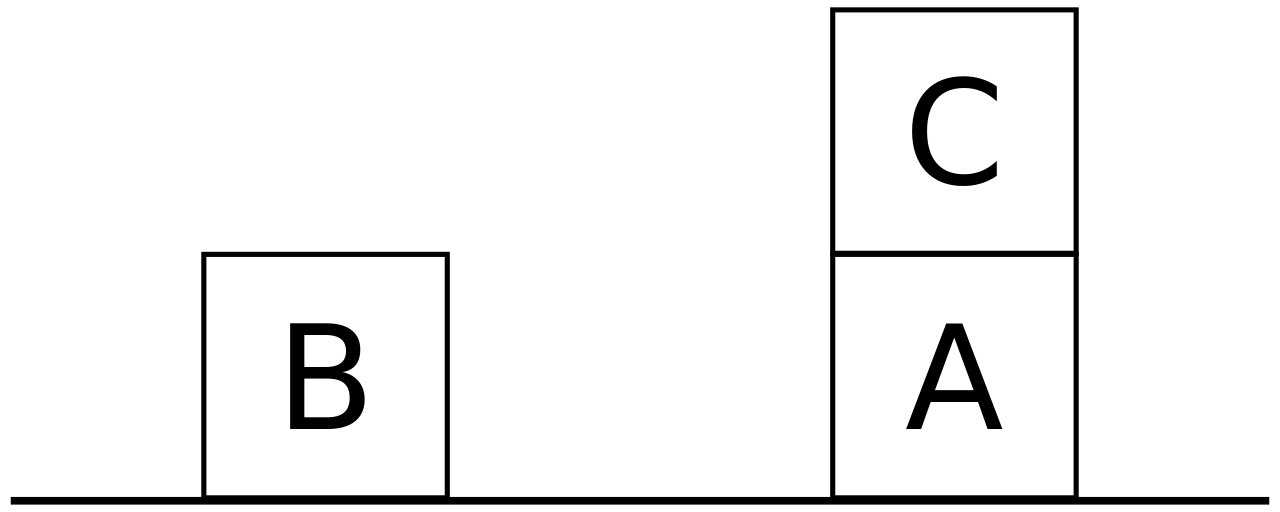
\includegraphics[width=0.5\textwidth]{1280px-Sussman-anomaly-1.svg.png}

}

  Un algoritmo di pianificazione lineare suddividerebbe il goal nei due sottogoal ``impila A su B'' e ``impila B su C''. 
  Tuttavia, soddisfare il primo goal nella maniera più efficiente porta il sistema nello stato descritto dalla figura seguente:

  {

    \centering

  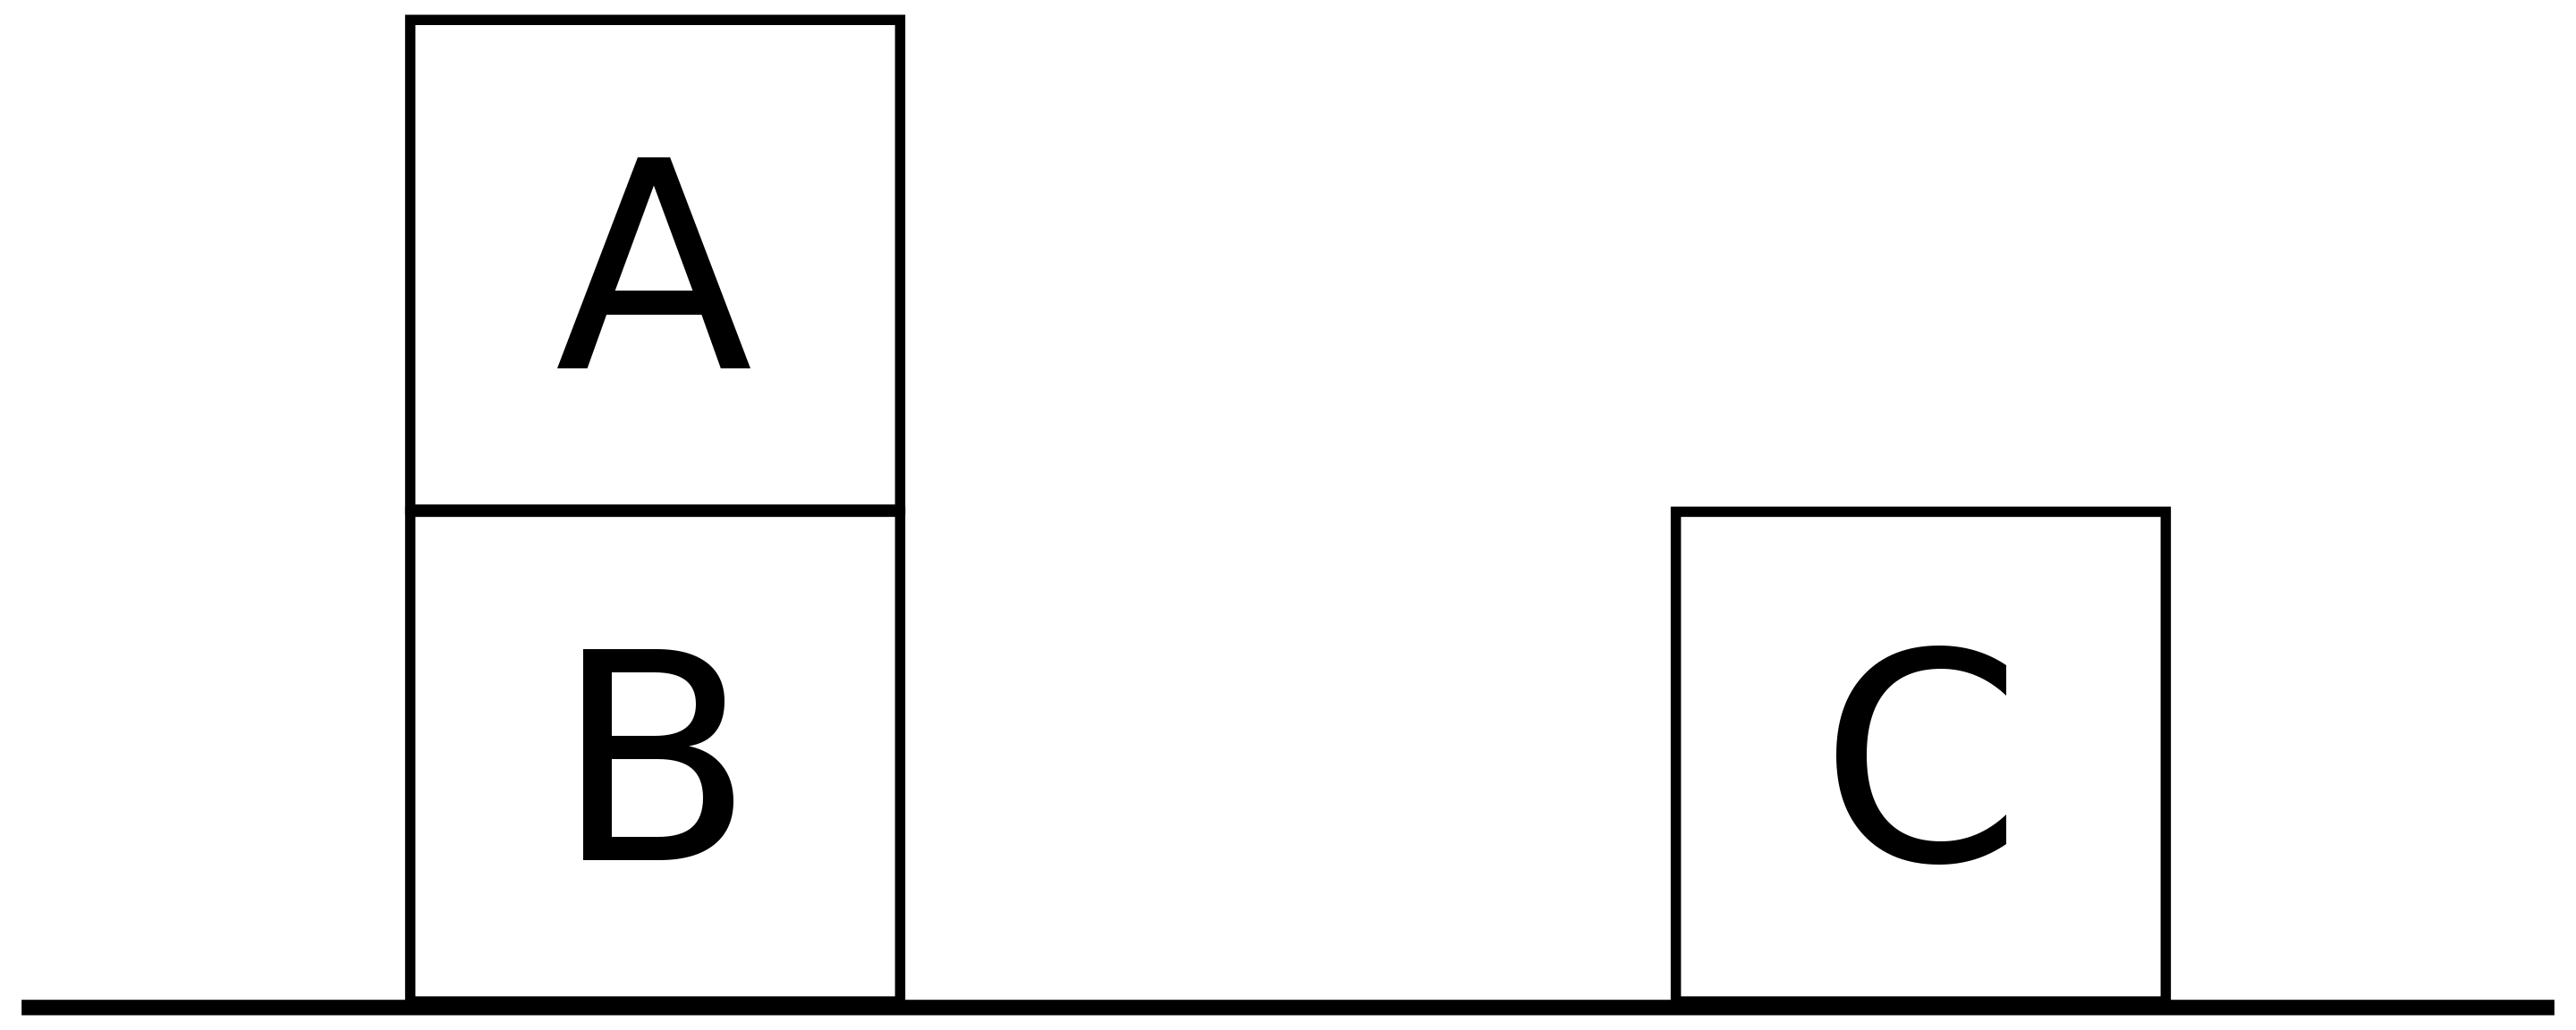
\includegraphics[width=0.5\textwidth]{2880px-Sussman-anomaly-2.svg.png}

}

  A questo punto, soddisfare l'altro sottogoal richiede di disfare quanto appena compiuto. 
  Se, al contrario, si soddisfa per primo il secondo sottogoal, ci si ritrova comunque in una situazione di stallo, la seguente:

    {

    \centering

  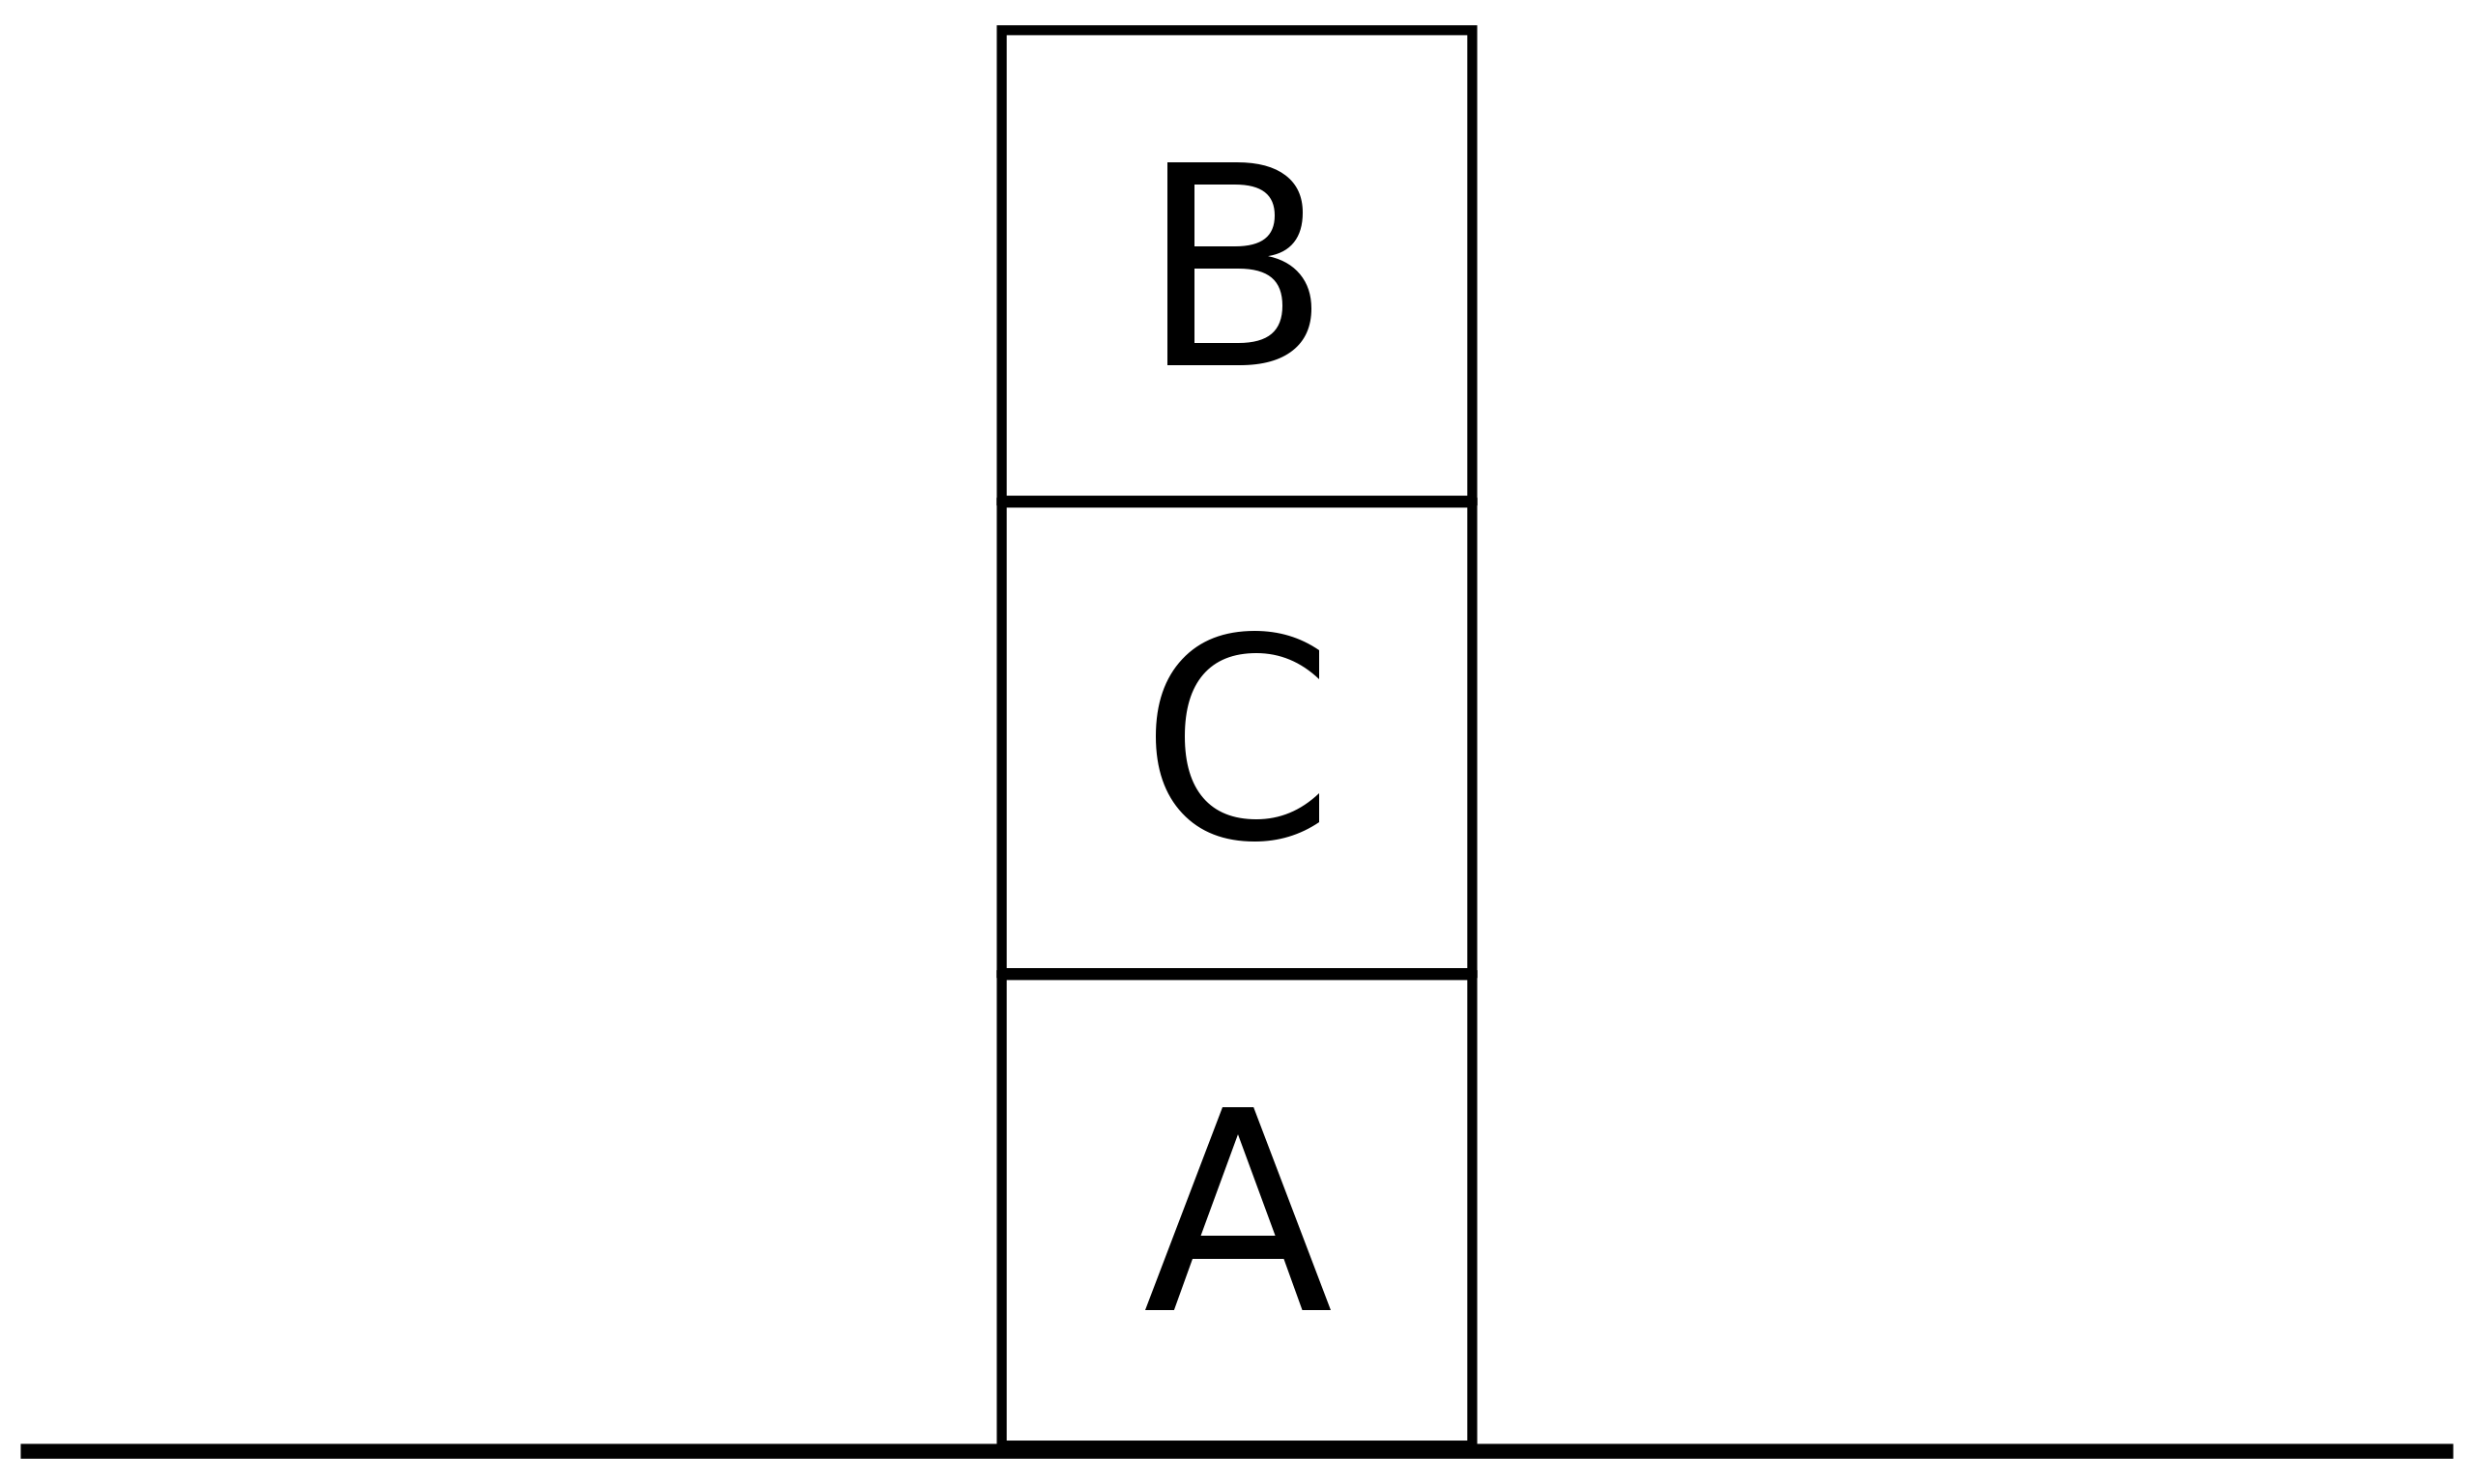
\includegraphics[width=0.5\textwidth]{2560px-Sussman-anomaly-3.svg.png}

}

È possibile arrivare al goal finale, ma non in maniera efficiente, il che mette in mostra una debolezza della pianificazione lineare. 

\end{solution}

\question Si spieghi cosa si intende per pianificazione classica e per pianificazione reattiva, illustrandone le
differenze, i vantaggi e gli svantaggi.
\begin{solution}
  La pianificazione è la definizione di un \emph{piano}, ovvero un insieme totalmente o parzialmente ordinato dai \emph{azioni} che portino lo \emph{stato} di un sistema da uno \emph{stato di partenza} a un \emph{goal} desiderato.

  La pianificazione classica, o \emph{offline}, prevede la definizione di un piano le cui azioni possono essere modificate in fase di pianificazione, ma non durante l'esecuzione del piano. 
  A questo fine, la pianificazione classica si avvale di una rappresentazione istantanea, detta \emph{snapshot}, dello stato corrente. 
  La pianificazione classica presume che solamente le azioni parte del piano modifichino lo stato di un sistema, che i cambiamenti di stato siano totalmente deterministici, che lo stato iniziale sia totalmente noto a priori e che le azioni vengano eseguite in modo atomico. 
  Queste assunzioni sono molto forti e raramente verificate in sistemi reali. 
  
  Per questo motivo si fa strada la pianificazione \emph{reattiva}, o \emph{online}, la quale considera il sistema come dinamico e non deterministico e può alterare il piano anche durante l'esecuzione, dato che continua a osservare lo stato del sistema anche in questa fase. 
\end{solution}
\question Si spieghi brevemente in cosa consiste la ricerca locale, vantaggi e svantaggi e si specifichi l’algoritmo dell’Hill-climbing, specificandone le caratteristiche.
\begin{solution}
  La ricerca locale è una classe di algoritmi di ricerca informata basata sull'esplorazione di ``soluzioni vicine'' a quella corrente che migliorino la situazione in termini di una funzione di valutazione $f(\cdot)$. 
Una ricerca locale richiede che sia definita una funzione $F(s) = N(s)$ che definisca $\forall s \in S$, essendo $S$ lo spazio delle soluzioni, una \emph{neighborhood} $N(s) \subset S$. 
Questa funzione determina la velocità di convergenza dell'algoritmo e solitamente è definita implicitamente dalle mosse possibili dato uno stato. 
  La funzione $f(\cdot)$ può non essere globalmente concava, quindi non è detto che la ricerca locale converga a un massimo globale.
  Se l'algoritmo converge a un massimo locale, più sono larghe le neighborhood e più è probabile che si tratti anche di un massimo globale, ma la complessità computazionale chiaramente aumenta. 
  L'algoritmo di hill climbing prevede che, a ogni passo, si scelga di muoversi verso lo stato nella neighborhood con il valore di $f(\cdot)$ più alto. 
  Questo tipo di algoritmo non gestisce un albero di ricerca ma tiene traccia solo dello stato corrente e dei suoi vicini; non avendo una ``visione globale'' può  convergere a un massimo locale di bassa qualità e non uscirne mai.
  Inoltre, la funzione $f(\cdot)$ può presentare \emph{altopiani}, zone molto ``piatte'' nelle quali gli stati vicini hanno tutti lo stesso valore e non è immediato decidere verso quale stato muoversi, o ``crinali'', stati con un valore maggiore ai quali non è possibile arrivare direttamente. 
  Una possibile soluzione a questi problemi è lanciare più volte l'algoritmo con condizioni iniziali casuali, salvare la soluzione migliore e restituirla dopo un certo numero di tentativi dettato dal tempo di computazione o dal numero di iterazioni. 
\end{solution}

\question Si spieghi cosa è un constraint graph per un problema di CSP e si definiscano i diversi livelli di
consistenza da quella di I grado (node consistency) al grado k.
\begin{solution}
  A differenza degli algoritmi di propagazione che propagano i vincoli in seguito a istanziazioni delle variabili coinvolte nel problema, le tecniche di consistena riducono il problema originale eliminando dai domini delle variabili i valori che non possono comparire in una soluzione finale.
  Per applicare tali tecniche bisogna rappresentare il problema come una rete di vincoli, chiamata grafo dei vincoli (constraint graph). I nodi del constraint graph rappresentano le variabili del CSP, mentre gli archi rappresentano i vincoli tra tali variabili.
  Si riportano di seguito i vari livelli di consistenza esistenti:
  \begin{itemize}

    \item Livello 1 - Node Consistency: la consistenza di grado 1 riguarda un solo nodo. Si dice che un nodo è consistente se per ogni valore $X_i \in D_i$  il vincolo unario $P(X_i)$ è soddisfatto.

    \item Livello 2 - Arc Consistency: la consistenza di grado 2 si ottiene da un grafo node consistent e riguarda 2 nodi del grafo. In particolare, questa consistenza verifica se un arco $A(i, j)$ che collega due nodi $X_i, X_j$ è consistente.
  Un arco $A(i, j)$ è consistente se per ogni valore $x \in D_i$, esiste almeno un valore $y \in D_j$ tale che il vincolo $P(i, j)$ tra $i$ e $j$ sia soddisfatto.

   \item Livello 3 - Path Consistency: la consistenza di gtrado 3 si ottiene partendo da un grafo arc consistente e riguarda 3 nodi del grafo. Un cammino $(X_i, X_j, X_k)$ è path consistente se, $\forall x \in D_i, y \in D_j$ che rispettano la node e la arc consistenza esiste un valore $z \in D_k$ che soddisfa i vincoli $P(i, k), P(k, j)$.
  La consistenza del vincolo unario $P(k)$ è garantita dalla node consistency della rete.

\item Livello $k$ - K-Consistency: scelti valori per ogni $(k-1)$-pla di variabili consistenti con i vincoli imposti dal problema, per ogni $k$-esima variabile si cerca un valore che soddisfa i vincoli tra tutte le $k$ variabili. Se tale valore esiste allore le $k$ variabili sono consistenti. In generale, se un grafo contenente $n$ variabili è $k$-consistente con $k < n$, allora per trovare una soluzione è necessaria una ricerca nello spazio restante.
  \end{itemize}
\end{solution}

\question Si descriva l’algoritmo di ricerca a costo uniforme, mostrando un semplice esempio. Se ne discutano le
proprietà (completezza, ottimalità, etc.)
\begin{solution}
	L'algoritmo di ricerca a costo uniforme, o algoritmo di Dijkstra, è un algoritmo di ricerca del cammino minimo sui grafi. 
  Si tratta di una ricerca in ampiezza nella quale i nodi non sono inseriti in una semplice coda ma in una coda di priorità, ordinata in modo tale che venga sempre estratto il nodo con la distanza minore dal nodo di partenza. 
  Quando dalla coda viene estratto il nodo di 
  La ricerca a costo uniforme è completa e ottimale, perché la prima volta che verrà espanso il nodo di arrivo la sua distanza dal nodo di partenza sarà minore di o uguale a quella di qualunque altro nodo in coda. 
  La complessità temporale della ricerca a costo uniforme è $O(b^{1 + C^*/\epsilon})$ essendo $C^*$ il costo totale della soluzione ottimale  e $\epsilon$ il minimo costo di un arco. 
	Lo pseudocodice per la ricerca a costo uniforme è il seguente:
  \begin{verbatim}
function dijkstra(graph, start, goal) returns solution or failure
  q <- new priority_queue
  dist_from_start <- new array
  parent <- new array
  for each u in graph do:
    dist_from_start(u) <- inf
    parent(u) <- null
  dist_from_start(start) <- 0
  parent(start) <- start
  push(q, start)
  while q is not empty do:
    u <- pop(q)
    if u = goal then return dist_from_start(u)
    for each child of u do:
      new_dist <- dist_from_start(u) + dist(u, child) 
      if new_dist <= dist_from_start(child) then:
        dist_from_start(child) <- new_dist
        parent(child) <- u
        push(q, (child, dist_from_start(child)))
  return failure
	\end{verbatim}
\end{solution}
\question Si descriva cos’è l'unificazione e il problema relativo all’assenza di occur check nel linguaggio Prolog.
\begin{solution}
  L'unificazione è un meccanismo che permette di calcolare una sostituzione al fine di rendere uguali due espressioni. Per espressione si intede un termine, un letterale o una congiunzione o una disgiunzione di letterali.
  Per una sostituzione $\theta$ = [X1/T1, X2/T2, ..., Xn/Tn] si intende un'insieme di legami di termini Ti a variabili Xi che rendono uguali due espressioni. L'applicazione di una sostituzione a un'espressione E, [E]$\theta$ produce una nuova espressione in cui vengono sostituite tutte le variabili di E con i corrispondenti termini.
  Esempio: Espressione 1: c(X, Y); Espressione 2: c(a, K). soluzione unificatrice: $\theta$ = [X/a, Y/K]. \newline
  Di solito si è interessati all'unificazione più generale tra due atomi, a patto che essi siano unificabili. A tal proposito esiste un algoritmo che calcola la MOST GENERAL UNIFIER o termina in tempo finito nel caso in cui i due atomi non sono unficabili:

  \begin{center}
    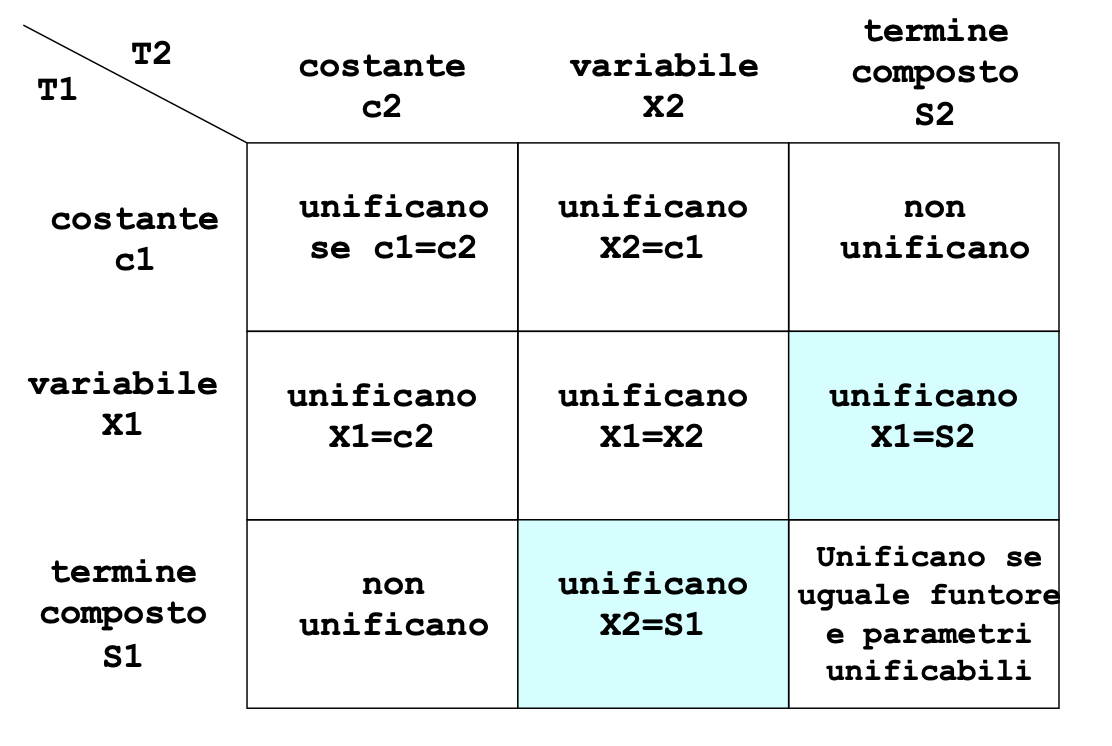
\includegraphics[width=0.5\textwidth]{AlgoritmoUnificazione.png}
  \end{center}

  L'unificazione tra una variabile X e un termine composto S è molto delicata: infatti è importante controllare che il termine composto S non contenga la variabile da unificare X. Cioè, per esempio, S(X) ed X non possono unificare.
  Questo controllo è chiamato \emph{occur check} e renderebbe quadratica la complessità dell'algoritmo di unificazione. Prolog omette l'operazione di occur check, tollerando l'inesattezza dell'algoritmo di unificazione. 
  Non da meno, la mancanza di occur check potrebbe inficiare anche la terminazione stessa dell'algoritmo. Ad esempio:

  [X/Y, X/f(X)]

  Chiaramente, due termini unificati con lo stesso termine sono uguali tra loro. Allora Y/f(Y), ma questo implica Y=f(f(f(f(...)))) e il procedimento non termina.

\end{solution}

\question Si descrivano gli algoritmi per CSP che utilizzano attivamente i vincoli nel corso della ricerca. Si descrivano in particolare gli algoritmi di propagazione visti (dal Forward Checking al Partial e Full Look Ahead), discutendone le differenze su un esempio.
\begin{solution}
Un CSP è un Constraints Satisfaction Problem, ovvero un problema di soddisfacimento vincoli in cui l'obiettivo è trovare uno stato del problema che soddisfi determinati vincoli.
Un CSP può essere approcciato mediante tecniche di consistenza o algoritmi di propagazione. Gli algoritmi d propagazione sono metodi di ricerca che tentano di prevenire i fallimenti attraverso il pruning (potatura) dell'albero decisionale. Essi utilizzano cioè le relazioni tra le variabili del problema, ovvero i vincoli, per ridurre lo spazio 
di ricerca prima di arrivare al fallimento. Rispetto allo Standard Backtracking, dunque, ad ogni assegnazione di variabile, gli algoritmi di propagazione aggiornano e controllano l'insieme di valori ammissibili (domini) di casciuna variabile ancora da istanziare (variabili future).

  \begin{itemize}

    \item Forward Checking: l'assegnazione di un valore ad una variabile ha ripercussioni sull'insieme dei valori disponibili per le variabili ancora libere. In questo modo i vincoli agiscono in avanti (forward) eliminando dai domini delle variabili future i valori incompatibili con la variabile appena istanziata. Se ad un certo punto della computazione il dominio associato ad una variabile risulta vuoto, il meccanismo di Forward Checking fallisce e si esegue backtracking.

    \item (Partial e Full) Look Ahead: come avviene nel Forward Checking, ad ogni istanziazione vien econtrollata la compatibilità dei vincoli contenenti la variabile appena assegnata con le precedenti (istanziate) e le successive (libere). Ma in più si guardano anche i vincoli tra coppie di variabili libere. Viene sviluppato cioè il cosiddetto look ahead che controlla l'esistenza, nei domini associati alle variabili ancora libere, di valori compatibili con i vincoli contenenti solo variabili ancora libere.
Quindi i domini associati a ogni variabile vengono ridotti propagando anche le relazioni tra coppie di variabili non ancora istanziate. Viene verificato che sia possibile una futura assegnazione consistente fra coppie delle variabili libere.
      Esistono due strategie per questa tecnica: Partial Look Ahead (PLA) e Full Look Ahead (FLA). Nel PLA si ha una propagazione dei vincoli tra la variabile Xh \emph{non ancora istanziata} e le variabili future $(X_{h+1}, X_{h+2},...,X_{h+n})$. 
      Nel FLA se $V_k$ è il valore appena assegnato alla variabile $X_k$, si ha una propagazione dei vincoli tra la variabile $X_h$, non ancora istanziata, e tutte le variabili non ancora assegnate, ossia le variabili $X_{k+1},...,X_{h-1},X_{h+1},...,X_n$.
  \end{itemize}
Adottando queste tecniche si hanno tre gradi di libertà: la scelta nell'ordinamento delle variabili, la scelta nell'ordine di selezione del valore da attribuire alla variabile corrente e la propagazione effettuata in ciascun nodo. Le prime due scelte riguardano le euristiche sulla strategia di ricerca (Es: MRV, most-constrained principle, least constraining principle).


\end{solution}

\question Si introduca il sistema STRIPS per la pianificazione, si spieghi come funziona e se ne evidenzino i limiti.
\begin{solution}
  Lo STanford Research Institute Problem Solving è un pianificatore automatico sviluppato nel 1971 che permette di rappresentare azioni con sintassi molto semplice ed efficiente. Esso campiona delle proprietà che valgono in un determinato istante/stato della realtà nei cosiddetti "fluent"; un esempio di fluent è \emph{ontable(c,s)}. 
  \newline Il linguaggio di STRIPS permette di:
  \begin{itemize}
    \item Rappresentare lo stato attraverso un insieme di fluent che valgono nello stato. Ad esempio: on(b,a), clear(b), clear(c), ontable(c), etc\dots
    \item Rappresentare il goal, similmente allo stato, attraverso un insieme di fluent. Si possono avere variabili, ad esempio: on(X, a)
    \item Rappresentare le azioni/regole mediante tre liste:
    \begin{itemize}
      \item PRECONDIZIONI: fluent che devono essere veri per applicare l'azione
      \item DELETE: fluent che diventano falsi come risultato dell'azione
      \item ADD: fluent che diventano veri come risultato dell'azione
    \end{itemize}
  \end{itemize}
  
  Un esempio di regola/azione è il seguente:
  \newline\emph{Move(X, Y, Z)}
  \newline PRECONDIZIONI: on(X,Y), clear(X), clear(Z)
  \newline DELETE LIST: clear(Z), on(X,Y)
  \newline ADD LIST: clear(Y), on(X,Z)
  \newline
  \newline NB: vale la cosiddetta \emph{STRIPS Assumption}: Tutto ciò che non è specificato nella ADD e DELETE list resta immutato.
  \newline Il pianificatore agisce secondo un algoritmo di ricerca nello spazio degli stati che funge planner lineare. Esso è basato su una ricerca backward e assume che lo stato iniziale sia completamente noto (Closed World Assumption).
  Come è possibile notare, fa uso di due strutture dati: uno stack di goal e una descrizione S dello stato corrente:

  \begin{verbatim}
  function strips
    s <- new stack
    push(s, congiunzione di goal finali)
    while s is not empty do:
      if top(s) = A and A theta sottoinsieme di  S then: 
        // si noti che A può essere un AND di goal o un atomo
        pop(s)
        esegui theta sullo stack
      else if top(s) = a then:
        R <- regola tale che a faccia parte di Addlist(R)
        pop(s)
        push(s, R)
        push(s, precond(R))
      else if top(s) = a[1] and a[2] and ... and a[n] then:
        for i from 1 to n do:
          push(s, a[i])
      else if top(s) = R then:
        pop(s)
        applica R su S
  \end{verbatim}
  
  Si noti che l'ordine con cui i sottogoal vengono inseriti nello stack rappresenta una punto di scelta non deterministica. La congiunzione rimane sullo stack e verrà riverificata dopo (interacting goals).
  Si riportano di seguito alcune considerazioni sull'algoritmo:
  \begin{itemize}
    \item Il goal è la prima pila di obiettivi.
    \item Si suddivide il problema in sottoproblemi: ciascuno per un componente dell'obiettivo originale. Tali sottoproblemi possono interagire.
    \item Abbiamo tanti possibili ordini di soluzione.
    \item Ad ogni passo del processo di risoluzione si cerca di risolvere il goal in cima alla pila.
    \item Quando si ottiene una sequenza di operatori che lo soddisfa la si applica alla descrizione corrente dello stato ottenendo una nuova descrizione S.
    \item Si cerca poi di soddisfare l'obiettivo che è in cima alla pila partendo dalla situazione prodotta dal soddisfacimento del primo obiettivo.
    \item Il procedimento continua fino allo svuotamento della pila.
    \item Quando in cima alla pila si incontra una congiunzione si verifica che tutte le sue componenti siano effettivamente soddisfatte nello stato attuale. Se una componente non è soddisfatta (problema dell’interazione tra goal) si reinserisce nella pila e si continua.
  \end{itemize}
I problemi che tipicamente si hanno con con questo algoritmo risiedono nel fatto che il grafo di ricerca è molto vasto (soluzione: strategie euristiche) e nell'interazione tra i goal: quando due o più goal interagiscono ci possono essere problemi di interazione tra le soluzioni (vedere domanda sull'anomalia di Sussman).
\end{solution}

\question Descrivere la ricerca A* e definire sotto quali condizioni tale algoritmo di ricerca trova la soluzione ottima.
\begin{solution}
  La ricerca A* è una versione informata della ricerca a costo uniforme nella quale i nodi non sono inseriti nella coda di priorità solo sulla base della loro distanza $g(x)$ dal nodo di partenza ma considerando invece il valore $f(x) = g(x) + h(x)$ essendo $h(x)$ una funzione euristica che stimi la distanza di un nodo $x$ dal nodo di arrivo. 
  La ricerca A* trova la soluzione ottima se l'euristica è ammissibile (v. domanda relativa). 
  Una condizione più forte dell'ammissibilità è la coerenza, che richiede che l'euristica rispetti la disuguaglianza triangolare, i.e. $h(x) <= d(x, y) + h(y)$ essendo $d(x, y)$ la distanza reale tra i nodi $x$ e $y$. 
  Ogni euristica coerente è ammissibile, ma non vale il viceversa. 
\end{solution}

\question 
Si spieghi brevemente il predicato predefinito Prolog \texttt{findall}.
\begin{solution}
  Il predicato \texttt{findall(X, P, L)} è un predicato del secondo ordine, ovvero che permette di conoscere l'insieme di elementi che soddisfano una data query. 
  \texttt{findall(X, P, L)} è vero se L è la lista di istanze di X tali che P sia vera. 
  Se non esistono X che soddisfino P, L è la lista vuota. 
\end{solution}
\question 
Si spieghi brevemente il predicato predefinito Prolog \texttt{call}.
\begin{solution}
  Il predicato predefinito \texttt{call(T)} tratta il termine T come un atomo e ne richiede la valutazione all'interprete Prolog. 
  Al momento della valutazione, T deve essere istanziato a un termine non numerico, contenente eventualmente delle variabili.
  Si può vedere l'interprete Prolog come un loop che chiama all'infinito \texttt{read(T), call(T)}. 
\end{solution}

\end{questions}


\textbf{Disclaimer}:  Questo documento può contenere errori e imprecisioni che potrebbero danneggiare sistemi informatici, terminare relazioni e rapporti di lavoro, liberare le vesciche dei gatti sulla moquette e causare un conflitto termonucleare globale.
Procedere con cautela.
Questo documento è rilasciato sotto licenza CC-BY-SA 4.0. \ccbysa
\end{document}

